\paragraph{Rate of covering of area}A stick of length L moves with velocity $\vec{v}$. $\vec{l}$ is perpendicular to stick and $| \vec{l} | = l$ and $\angle\vec{l}\vec{v}=\theta$


\begin{center}
	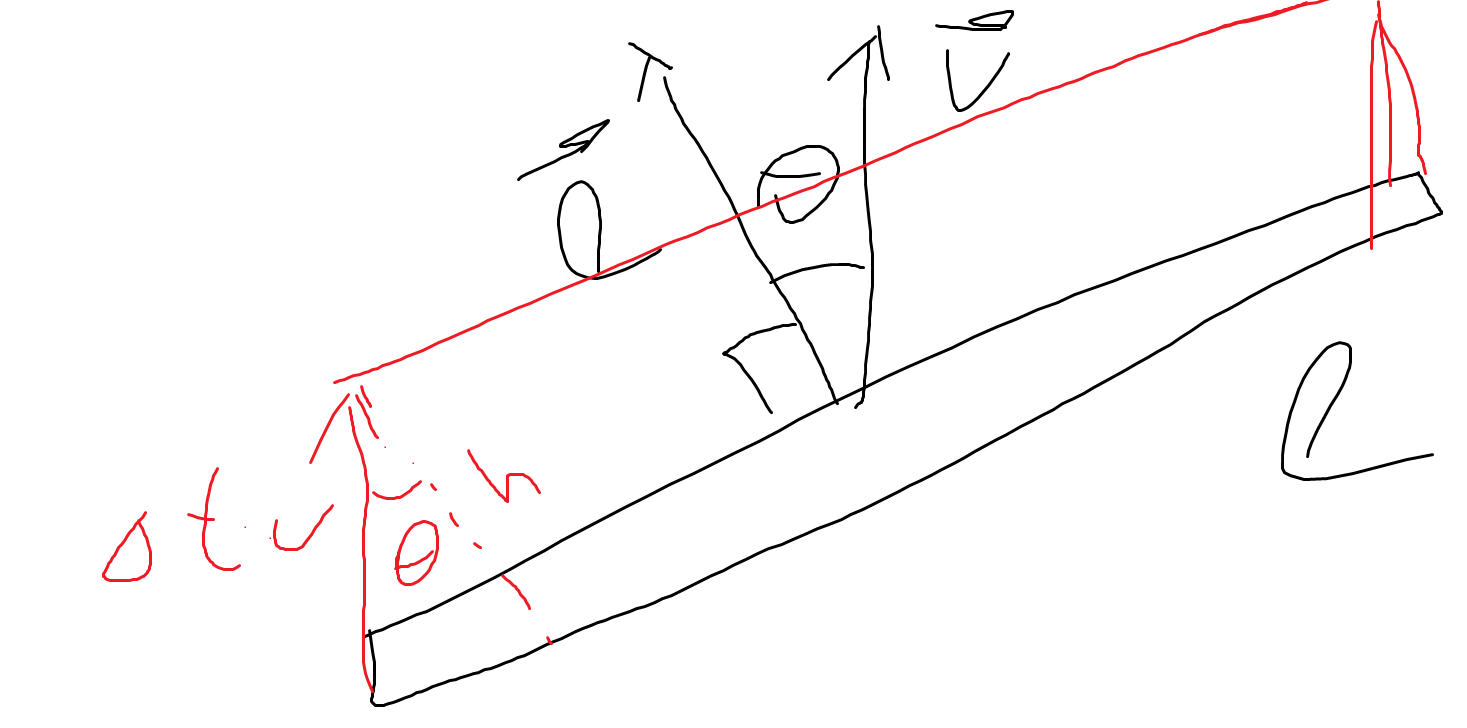
\includegraphics[width=0.4\linewidth]{./lect3/pic1.png}
\end{center}

What is area covered by a stick in time $\Delta t$?

$$dA = hl = \Delta tv \cos \theta l $$
$$\Delta t \rightarrow dt $$
$$\frac{dA}{dt} = vl \cos \theta = \vec{v} \cdot \vec{l}$$

\paragraph{Rate of covering of volume} Surface of area $\vec{S} = \vec{a} \times \vec{b}$.

\begin{center}
	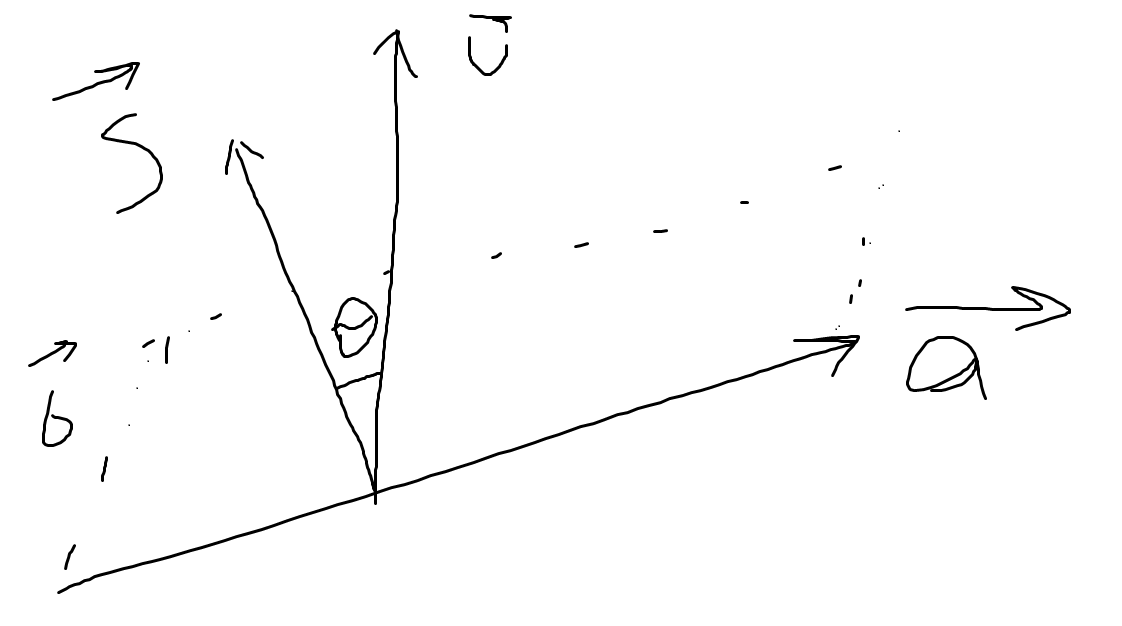
\includegraphics[width=0.3\linewidth]{./lect3/pic2.png}
\end{center}

Volume is 
$$dV = (vdt) S \cos \theta $$
$$\frac{dV}{dt} = vS \cos \theta = \vec{v} \cdot \vec{S}$$


What is mass of air covered by surface per time?
$$\frac{d m_{air}}{dt}= V \cdot \rho_{air} = \vec{S} \cdot \vec{v} \rho_{air} $$
$$\frac{d m_{air}}{dt} = \dot{m}_{air} = \vec{S} \cdot \vec{v} \rho_{air} = \vec{S} \cdot \vec{\Phi_{air}}$$

$\vec{\Phi_{air}}= \left[\frac{kg}{m^2 sec}\right] =$ flux of mass of air.


\paragraph{Torque(moment of force)}


\begin{center}
	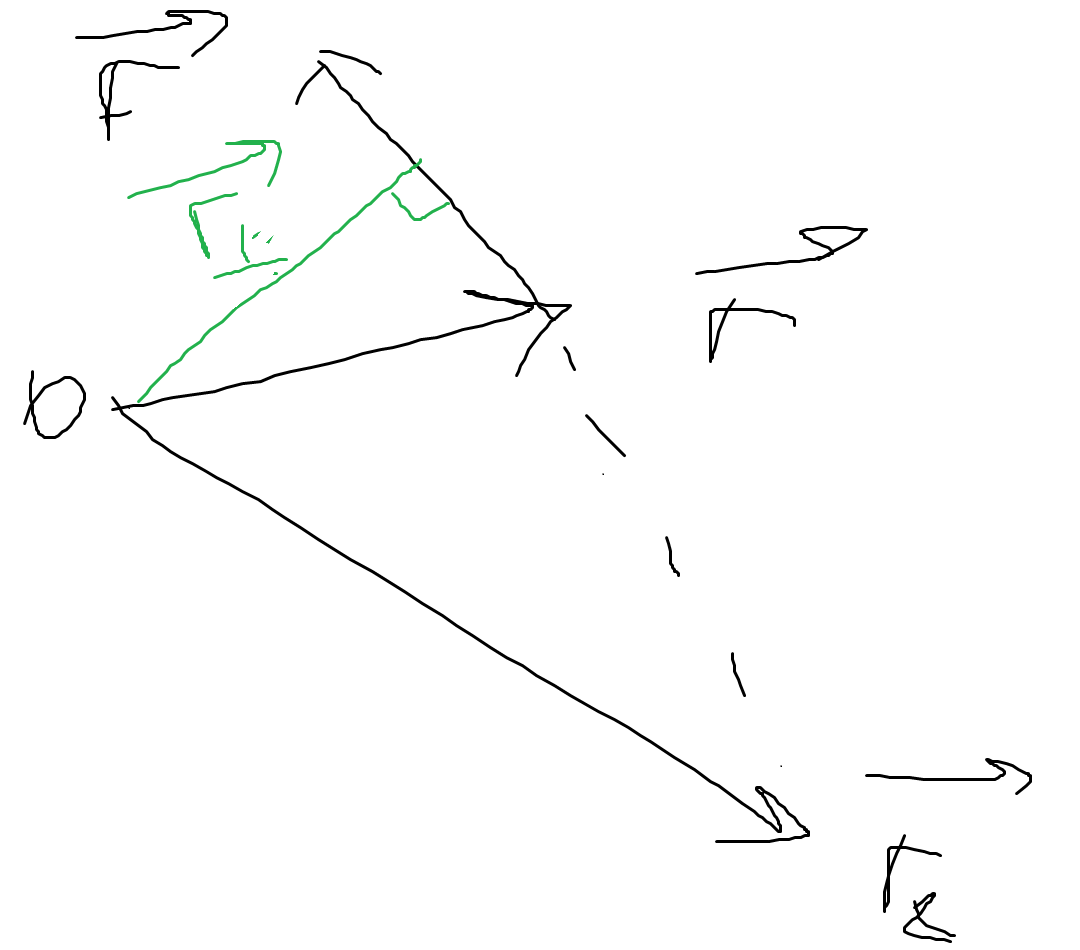
\includegraphics[width=0.3\linewidth]{./lect3/pic3.png}
\end{center}

$\vec{N} = \vec{r} \times \vec{F} \\
\vec{F} = \left[\frac{kg m}{s^2}\right] \\
\vec{r} = \left[m\right]\\
\vec{N} \left[\frac{kg \cdot m^2}{s^2}\right]$

$$\vec{N} = \vec{r} \times \vec{F} =  \vec{r}_1 \times \vec{F} = \vec{r}_{\perp} \times \vec{F} $$

\section{Derivatives of vector}

Derivative of position of body by time is velocity

$$\vec{v} = \frac{d\vec{r}}{dt} = \lim_{\Delta t \to 0} \frac{\Delta\vec{r}}{\Delta t}$$


\begin{center}
	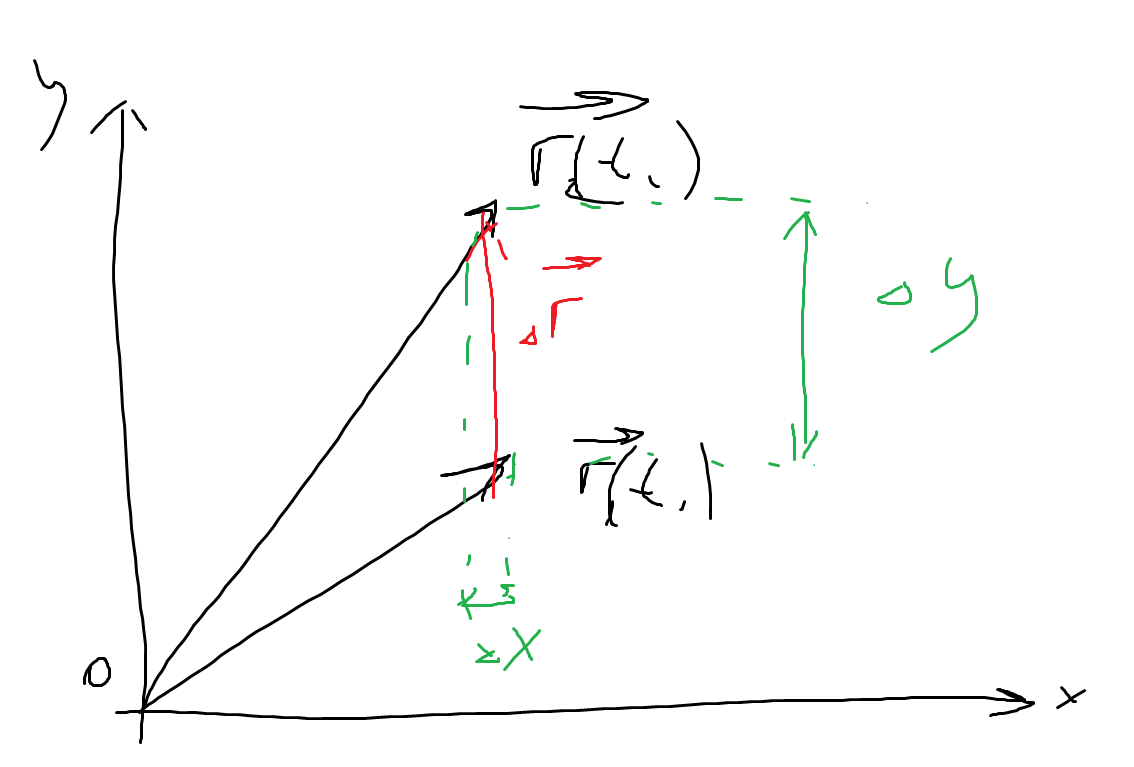
\includegraphics[width=\linewidth]{./lect3/pic4.png}
\end{center}

$$\Delta \vec{r} = \vec{r}(t_2) - \vec{r}(t_1) $$
$$\vec{v} = \frac{d \vec{r}}{dt} = \frac{dx}{dt}\hat{x} + \frac{dy}{dt}\hat{y} + \frac{dz}{dt}\hat{z} $$
$v = | \vec{v} | = \sqrt{v_x^2 + v_y^2 + v_z^2}$ where $v_x = \frac{dx}{dt}$

\textbf{When coordinate system doesn't change with time}

\subsection{Coordinate system changing in time}

\begin{center}
	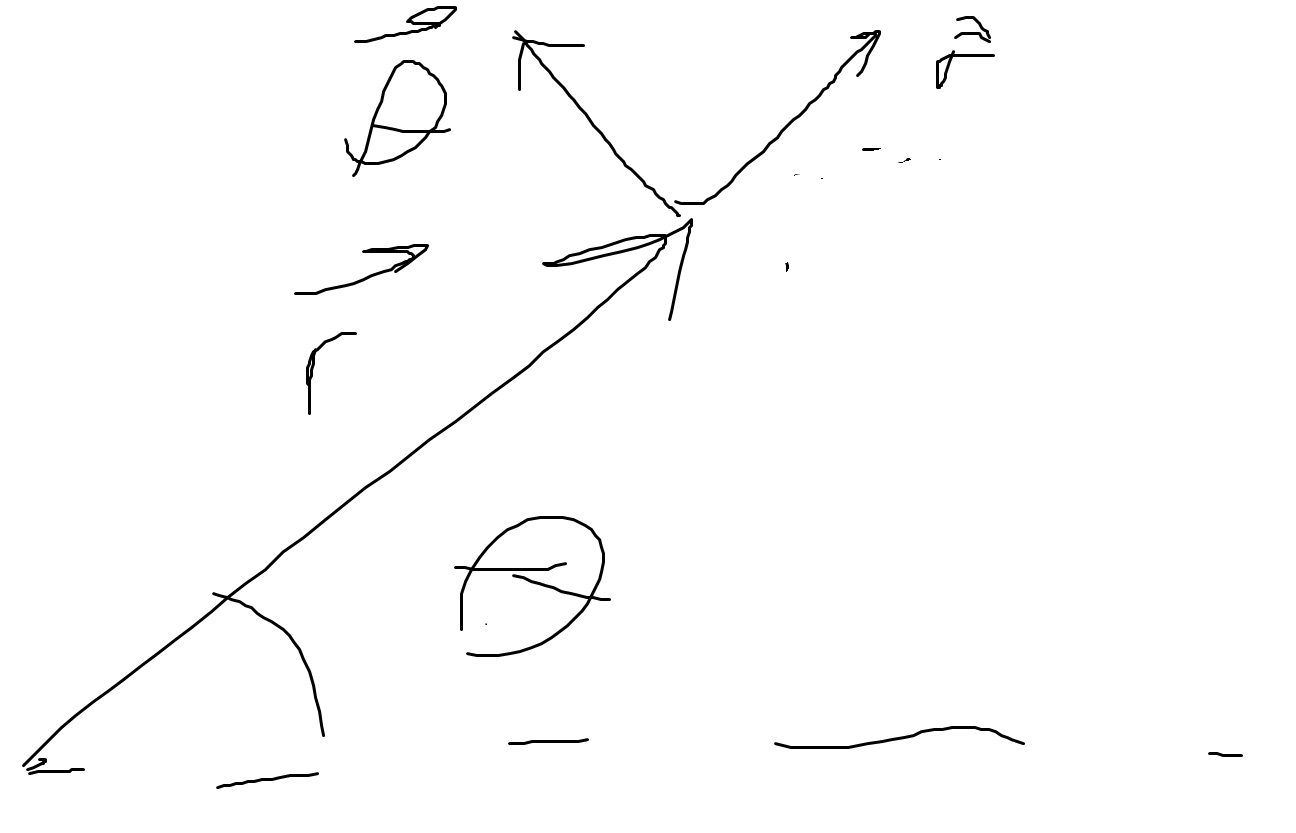
\includegraphics[width=0.25\linewidth]{./lect3/pic5.png}
\end{center}

$$\vec{r} = r \cdot \hat{r} $$
\begin{align*}
\left(\mbox{\FiveStarOpen}\right) &\vec{v} = \frac{d\vec{r}}{dt}= \frac{d}{dt} (r\hat{r}) = \frac{dr}{dt}\hat{r} + r \frac{d\hat{r}}{dt}
\end{align*}

\paragraph{Circle movement}

\begin{center}
	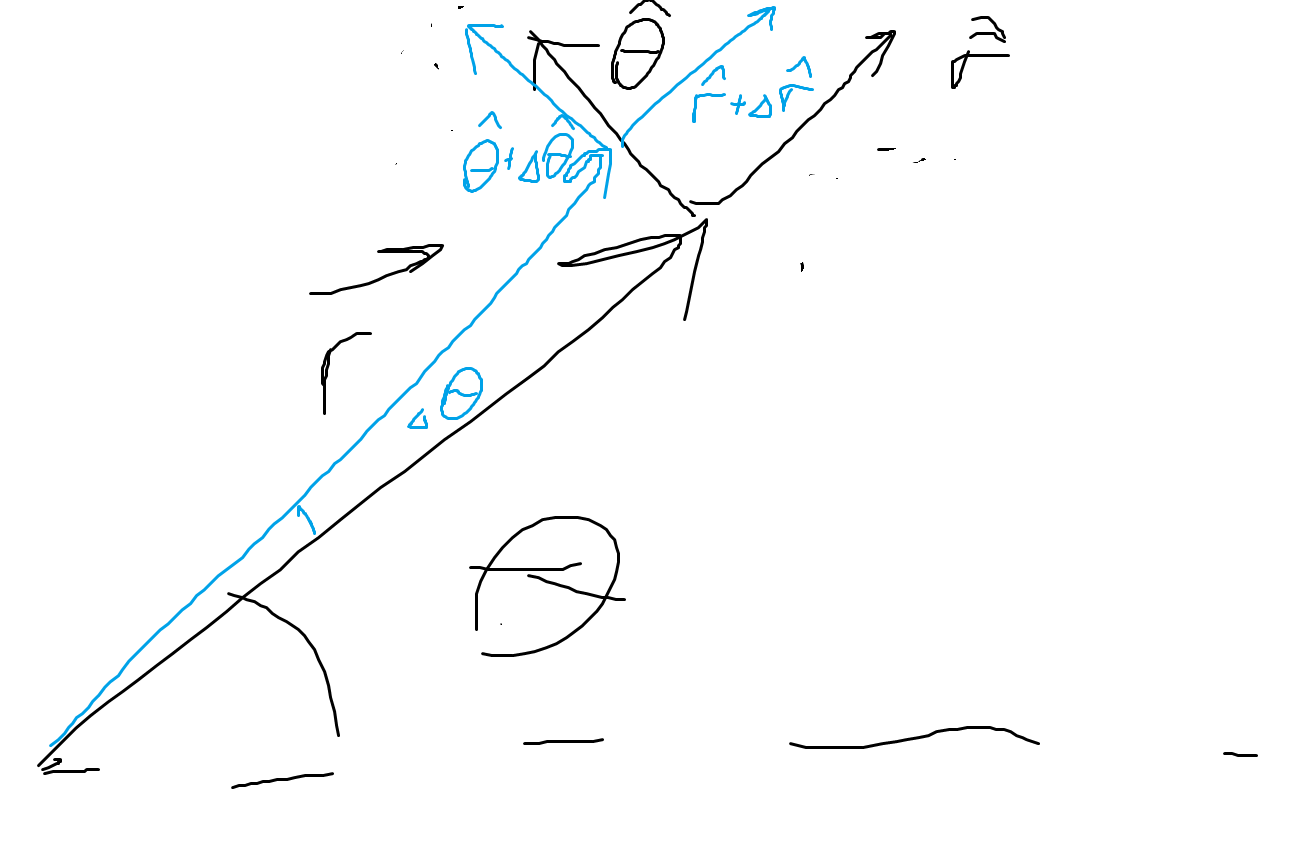
\includegraphics[width=0.4\linewidth]{./lect3/pic6.png}
\end{center}

Lets find $\Delta \hat{r}$ and $\Delta \hat{\theta}$. Move parallel beginnings of $\Delta \hat{r}$ to beginning of $\hat{r}$:

\begin{center}
	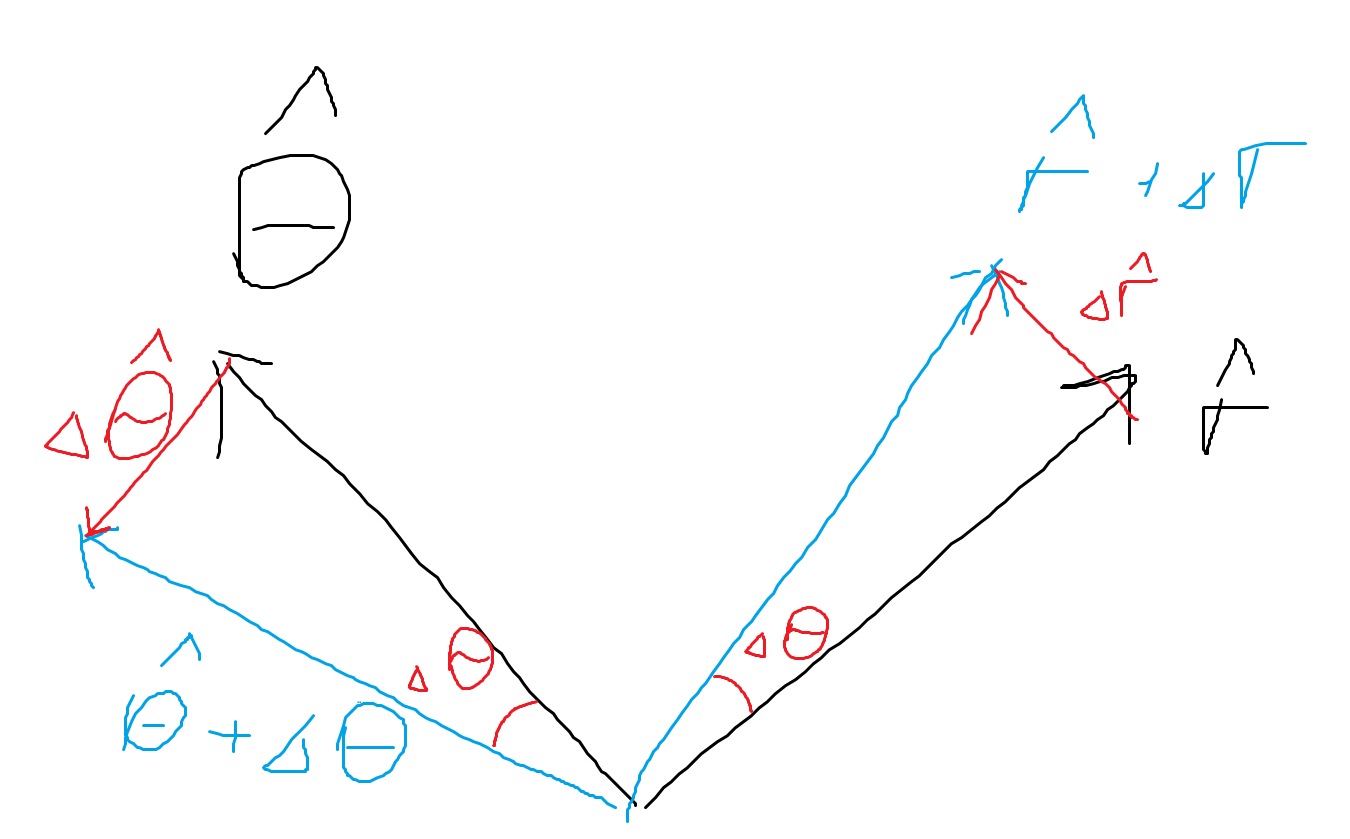
\includegraphics[width=0.4\linewidth]{./lect3/pic7.png}
\end{center}
$$\sin \alpha \simeq \alpha$$

$$\Delta \hat{r}  \parallel \hat{\theta} \perp \hat{r} $$
$$| \Delta \hat{r} | = | \hat{r} | \sin{\Delta \theta} = 1 \cdot \Delta \theta$$


Let's show that change in $\hat{r}$ is perpendicular to $\hat{r}$:

$$\frac{d}{dt}(1) = 0 = \frac{d}{dt}(\hat{r}\cdot\hat{r}) = \frac{d\hat{r}}{dt} \cdot \hat{r}+ \hat{r} \cdot \frac{d\hat{r}}{dt}$$
$$\hat{r} \cdot \frac{d\hat{r}}{dt} = 0$$
$$\hat{r} \perp \frac{d\hat{r}}{dt}$$

So $\Delta \hat{r} = (\Delta \theta) \cdot \hat{\theta}$
$$\frac{\Delta \hat{r}}{\Delta t} = \frac{(\Delta \theta) \cdot \hat{\theta}}{\Delta t}$$

When $\Delta t \to 0$

$$\frac{d \hat{r}}{d t} = \frac{(d \theta) \cdot \hat{\theta}}{d t}$$

Denote:

$$\omega = \frac{d \theta}{dt} $$

\begin{align*}
\left(\star\right) & \dot{\hat{r}} = \frac{d\hat{r}}{dt} = \omega \hat{\theta}
\end{align*}

\paragraph{$\Delta \hat{\theta}$} Similarly, direction of $\Delta \hat{\theta}$ is $-\hat{r}$ and $| \Delta \hat{\theta} | = \Delta\theta$

\begin{align*}
(\star\star) & \dot{\hat{\theta}} = \frac{d \hat{\theta}}{d t} = - \frac{d \theta}{dt} \hat{r}  = - \omega \hat{r}
\end{align*}